\section{Basics of traceability}\label{sec:BasicsOfTraceability}
Historically the research on traceability in software engineering originates from requirement engineering (RE). 
The question is: given a discrete set of requirements, how can one validate or even prove that all requirements are met? 
And more importantly on what information can one base such validation? 

The idea to solve this problem came through observation on typical product development processes where a raw vision is transformed to concrete requirements, requirements are transformed to architecture and architecture is transformed to a final implementation. 
Due to the incremental and iterative nature of such processes it is reasonable to assume that engineering activities might leave \textit{traces} which reflect the performed activity and the past state of the modified artifact.

Later traceability became of more interest to the MDE community. 
The purpose of traceability here did not much differ from its purpose in requirement or software engineering. 
We just change our perspective on how we see and describe engineering processes. 
Usually we try to regard artifacts as models of some kind at best specified by meta-models, and activities are seen as also well defined model-transformations. 
On top of that MDE is strongly interested in the automation of engineering processes.

Winkler and von Pilgrim compiled a complete survey on traceability where origins and differences in both fields can be explored in more detail \cite{TraceabilitySurvey}. 
This section is strongly based on their work.


\subsection{Traceability definitions}
Traceability is subject of various research fields, hence there is no standard definition on what traceability actually is. 
The introductory citation is from Lago et al. \cite{ScopedTraceability} and states the following: 
\textit{''Traceability is the ability to describe and follow the life of a software artifact and a means for modeling the relations between software artifacts in an explicit way''}. 
This definition is a good starting point if one wants to grasp what traceability is about because it is based on the life-cycle of artifacts and their relationships which has a nice intuitive notion. 
However, there is a weakness, it is not clear whose ability it should be. Other more technical definitions of traceability are given by the IEEE \cite{IEEEGlossary}:
\begin{enumerate}

\item 
\label{item:IEEEDef1}
\textit{The degree to which a relationship can be established between two or more products of the development process, especially products having a predecessor-successor or master-subordinate relationship to one another.}

\item 
\label{item:IEEEDef2}
\textit{The degree to which each element in a software development products establishes its reason for existing.}

\end{enumerate}
Here, traceability is not seen as an ambiguous ability, on the contrary it is stated as a hopefully measurable degree of relationships. 
Moreover in definition \ref{item:IEEEDef2} product elements are made accountable for their own traceability.


\subsubsection{traces}
Vital to traceability is the idea that engineering activities leave traces. 
Such traces may appear in form of meta-information describing hard facts like \textit{what} happened, \textit{who} did something or \textit{when} something happened. 
Opposing that traces also may appear as \textit{''... (non-) material indication or evidence ...''} \cite{OED} on \textit{why} or \textit{how} something happened. 

For example version control systems automatically record the user, modification date and the modification itself committed for a given artifact.
Additionally a commit-message is passed alongside which hopefully gives some insights on the stored changes.
These messages could refer to a customer interview, a discussion under colleagues or technical research to establish some reason on the modification. 
Such conversations are usually not transcribed, hence they are considered soft traceability information.
Note: the modification itself is also considered to reflect such non-material traceability information, although this data is hard to obtain unless there is explicit documentation like sufficient doc-comments or commit-messages.

Following this separation in hard and soft fact traces Pinheiro \cite{Pinheiro} defines a classification which somewhat resembles the separation commonly used on requirements:
\begin{itemize}

\item
\textbf{Functional traces:}
Traces existing due to well defined transformations. Such transformations produce traces as by-products like revision numbers in version control systems. Or traces that may be obtained by analyzing the transformation input, output and rules. In short, these traces have to obey some sort of formalism.

\item
\textbf{Non-Functional traces:}
Traces which cover \textit{''reason, context, decision, and technical''} aspects. I.e. explaining the informal interpretation of MUST and SHOULD in requirements.

\end{itemize}

\subsubsection{traceability links}
The IEEE \cite{IEEEGlossary} defines a trace as a record \textit{''To establish a relationship between two or more products of the development process; for example, to establish the relationship between a given requirement and the design element that implements that requirement.''}. 
The frequent notion of relationships describing or supporting traceability leads to the concept of \textit{traceability links}.
These links can be seen as a more technical description of traces as they are stated to be instances of  n-ary, multi-directional relations, although they are not named by the IEEE Glossary like traces and are often used as synonyms for one another \cite{TraceabilitySurvey}.
This can be misleading in environments which are not not strongly modeled where traceability links seem to not cover simple meta-data.

\begin{figure}
\centering
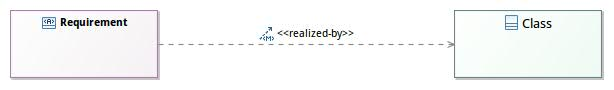
\includegraphics[width=\textwidth]{SimpleRealizationTraceabilityLink.jpg}
\caption{Requirement realization link}
\label{fig:RequirementRealizationLink}
\end{figure}

A simple example for traceability links is shown in Figure \ref{fig:RequirementRealizationLink} where the realization of a requirement by a class is denoted. 
However, this is a minimal example, in real-life the relation might need a higher arity to add constrains and test cases in order to confirm realization.

There are also categorizations on traceability links mostly considering the phase or abstraction nature.
For requirements engineering Gotel and Finkelstein use a big phase classification differentiating between \textit{pre- and post- requirement specification traceability} \cite{GotelFinkelstein}.
On the other hand Ramesh and Edwards distinct between \textit{horizontal and vertical traceability} \cite{RameshEdwards}.
Figure \ref{fig:RequirementRealizationLink} exemplifies vertical traceability as realization is a relation between abstraction layers.

Similar to these classifications there is \textit{pre-, intra- and post model traceability} by Paige et al. for MDD considering traceability between the first non-model artifacts and the first model, traceability during model-refinement and traceability between the final model and generated artifacts \cite{TraceabilitySurvey}.

Till now we introduced the mere concept of traceability which is far from applicable.
To make actually use of traces and traceability links we need do define schemes in RE or meta-models in MDD which also may vary with their targeted domain.
Traceability meta-models will be covered in a later section.


\subsection{Traceability objectives}
Another thing we like to point out besides the introduction to the rather theoretical concept of traceability is the motivation behind all this. 
Winkler and von Pilgrim \cite{TraceabilitySurvey} identified several objectives where traceability might be of great help. 
Figure \ref{fig:TraceabilityObjectives} depicts traceability objectives sorted by the research field they originated from. 
However most objectives found in requirements engineering can also be considered important to the MDD community. 
Additionally some objectives already correspond directly, i.e. \textit{Estimating change impact} and \textit{Change impact analysis} do not differ at all regarding their purpose. 
Given sufficient traceability information in form of traces and traceability links one can simulate changes top-down to the final model and estimate their impact on metrics like quality, performance, cost, etc. 
The only difference between RE and MDE here lies in the propagation of changes. 
Where in RE changes are considered to be propagated manually, MDE uses automation. 
Although nowadays RE also relies on tool support.

\begin{figure}
\centering
%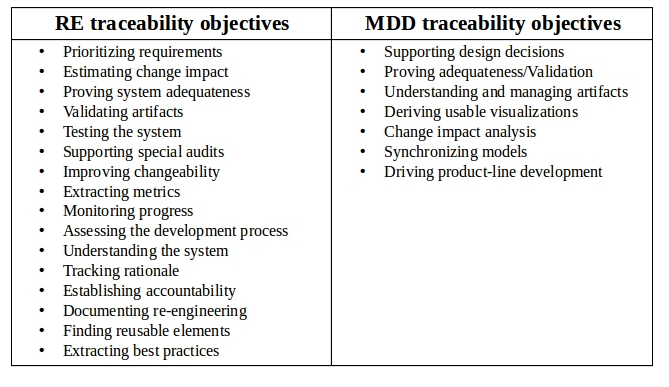
\includegraphics[width=\textwidth]{TraceabilityObjectives.jpg}
\begin{tabular}{|c|c|}
\hline
\begin{minipage}[t][][c]{0.5\textwidth}
\centering
\textbf{RE Traceability Objectives}
\end{minipage}

&

\begin{minipage}[t][][c]{0.5\textwidth}
\centering
\textbf{MDE Traceability Objectives}
\end{minipage}

\\\hline

\begin{minipage}[t][][c]{0.5\textwidth}
\vspace{0.1cm}
\begin{itemize}
\renewcommand{\labelitemi}{$\bullet$}

\item Prioritizing requirements 
\item Estimating change impact 
\item Proving system adequateness 
\item Validating artifacts 
\item Testing the system 
\item Supporting special audits 
\item Improving changeability 
\item Extracting metrics 
\item Monitoring progress 
\item Assessing the development process
\item Understanding the system 
\item Tracking rationale 
\item Establishing accountability 
\item Documenting re-engineering 
\item Finding reusable elements 
\item Extracting best practices 

\end{itemize}
\vspace{0.1cm}
\end{minipage}

&

\begin{minipage}[t][][c]{0.5\textwidth}
\vspace{0.1cm}
\begin{itemize}
\renewcommand{\labelitemi}{$\bullet$}

\item Supporting design decisions
\item Proving adequateness/Validation
\item Understanding and managing artifacts
\item Deriving usable visualizations
\item Change impact analysis
\item Synchronizing models
\item Driving product-line development

\end{itemize}
\vspace{0.1cm}
\end{minipage}

\\\hline

\end{tabular}
\caption{Traceability Objectives identified by Winkler and von Pilgrim \cite{TraceabilitySurvey}}
\label{fig:TraceabilityObjectives}
\end{figure}

Other corresponding objectives are \textit{Proving system adequateness}/\textit{Validating artifacts} and \textit{Proving adequateness/Validation}. 
If end-to-end traceability from early artifacts to the final implementation is achieved, one cannot only use traces to identify incompleteness (again top-down), it is also possible to check for requirement coverage (bottom-up).
This is especially beneficial for the use case to attest customers that the system specification is met and not exceeded.

Besides these product centric objectives which mainly address maintainability and soundness concerns of a completed project, there are also objectives to support the development process itself.
Such are \textit{Monitoring progress} and \textit{Establishing accountability} where project management can leverage end-to-end traceability to determine if a milestone is reached or who to blame if not. 

Eventually we can learn from collected traceability data during a project revision while \textit{Extract Best Practices} to support future design decisions. 



